%!TEX root = these.tex

\chapter[Contexte/Besoin/Applications]{plif}
\minitoc
\label{chap1}
\cleardoublepage

	\section{Contrôle de l'espace aérien}
	La figure~\ref{fig:airtraffic} représente un écran de contrôle du trafic aérien. Les trajectoires des avions sont (normalement) légèrement courbées ou rectilignes, ce qui les rend particulièrement prévisibles, et donc facilite considérablement la tâche de sélection, comme nous le verrons en détail plus loin. Cependant, selon le niveau de zoom et la quantité d'informations contextuelles affichées sur l'écran, le niveau d'occultation peut devenir très important. La vitesse des cibles dépend également du niveau de zoom, mais dans une relation inverse : plus l'échelle est grande, plus les mouvements des avions seront lents sur l'écran.
	
	\subsection{Applications civiles}
	Quantitativement, un avion de ligne atterrit à environ 250~km/h et ne dépasse pas 1000~km/h. Ses changements de direction sont très progressifs, généralement de l'ordre de deux degrés par seconde. Ils sont peu fréquents et généralement prévisibles car ils ont pour but d'emprunter des couloirs aériens, ou des trajectoires d'approche imposées aux abords des aéroports.

	\paragraph{}
	Il n'en va toutefois pas de même pour les hélicoptères, qui peuvent faire demi-tour en environ quatre secondes, voire moins. Cependant, les modèles civils dépassent rarement les 300 km/h. La fréquence des changements de direction dépend considérablement de la mission, elle peut être faible pour un simple transport d'un point A vers un point B, auquel cas la trajectoire de l'hélicoptère va tendre vers la ligne droite, ou assez importante dans le cas d'un hélicoptère de police fournissant une assistance aérienne pendant une course-poursuite.
	
	\subsection{Applications militaires (surveillance de l'espace aérien)}
	Les aéronefs militaires présentent des caractéristiques beaucoup plus variables, dans des intervalles nettement plus grands. La vitesse d'un avion de chasse, par exemple, peut atteindre 3000~km/h~\cite{mig31}. Il est beaucoup plus difficile d'obtenir des données chiffrées sur la maœuvrabilité de tels engins, mais il est du moins clair qu'un avion de chasse moderne peut changer de direction beaucoup plus brutalement qu'un avion de ligne, et certaines sources non officielles font état de capacités de l'ordre de 35\textdegree{}/s pour les meilleurs. La fréquence maximale à laquelle un avion peut changer de direction est également difficile à connaître avec certitude, mais une simple observation d'une démonstration en vol permet d'estimer que cette valeur est, grossièrement, de l'ordre d'un changement par seconde environ~\cite{rafdemo}. Indépendamment des capacités techniques des avions militaires, leurs missions peuvent précisément imposer la recherche de l'imprévisibilité (par exemple pour éviter les tirs ennemis) ce qui n'est généralement pas le cas dans le civil.
	
	\begin{figure}[ht]
		\centering
		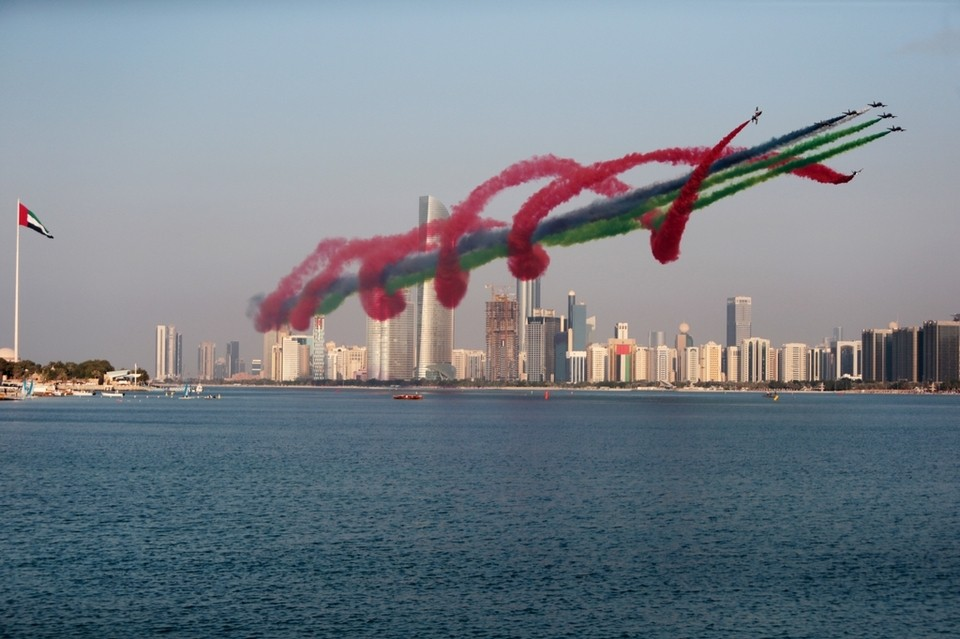
\includegraphics[width=\textwidth]{figures/AlFursan}
		\caption{La patrouille acrobatique émiratie \emph{Al Fursan}, avec ses trajectoires entremêlées mises en évidence par des traînées de fumée colorées. Crédit : The National UAE (\url{http://www.thenational.ae}).}
		\label{fig:swarm}
	\end{figure}
	
	\paragraph{}
	De même, les hélicoptères militaires sont plus agiles que leurs homologues civils, sans qu'il soit aisé de quantifier cette différence. Comme pour les avions, leur comportement est susceptible d'être  Ils sont ausssi légèrement plus rapides, de quelques dizaines de km/h, notamment en piqué. Comme pour les avions, leurs missions impliquent souvent des trajectoires moins prévisibles.
	
	\paragraph{}
	Le cas des drones aériens, c'est-à-dire des aéronefs sans pilote embarqué (télécommandés ou autonomes) est peut-être le plus hétérogène. On trouve en effet des drones de très petite taille, mais aussi des modèles de plusieurs tonnes~\cite{reaper}. Leurs modes de sustentation sont très divers, leurs moyens de propulsion varient également, et de fait, leurs caractéristiques de vol sont extrêmement variables, des plus petits engins extrêmement manœuvrables jusqu'au plus gros, qui se comportent comme des avions. Au-delà de leurs caractéristiques de vol, certains drones sont délibérément conçus pour être utilisés en grandes quantités, en essaims~\cite{locust, alonso2016distributed, saska2014autonomous}, notamment pour submerger l'ennemi par le nombre. Cela implique une densité de cibles potentiellement très importante, avec les niveaux d'occultation qui en découlent.
	
	\begin{figure}[ht]
		\centering
		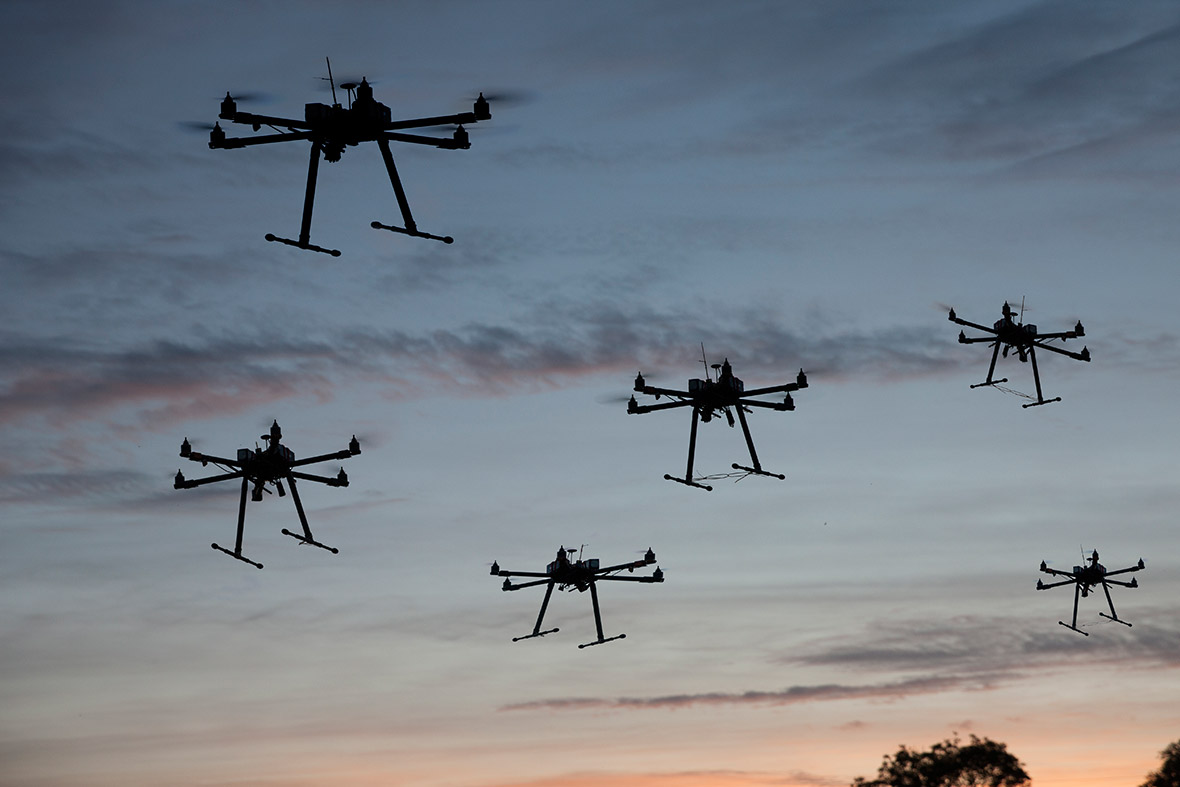
\includegraphics[width=\textwidth]{figures/swarm}
		\caption{Petit essaim de drones aériens. Crédit : International Business Times (\url{http://www.ibtimes.co.uk}).}
		\label{fig:swarm}
	\end{figure}
	
	\paragraph{}
	Dans une certaine mesure, le contrôle du trafic de drones est également un enjeu pour le domaine civil, car ils peuvent évoluer (légalement ou non) près des aéroports. Cette pratique peut représenter un risque de sécurité, et des arrêtés ont été pris par le Ministère de l'écologie et du développement durable pour les prévenir, comme le rappelle notamment l'Union des Aéroports Français~\cite{dronesuaf}.
	
	\paragraph{}
	La surveillance de l'espace aérien concerne également divers types de missiles (de croisière, balistiques, etc.). Leurs caractéristiques détaillées sont généralement au moins aussi secrètes que celles des avions de chasse, mais on sait néanmoins qu'ils peuvent être à la fois hypersoniques (c'est-à-dire dépasser Mach~5) et manœuvrables à de telles vitesses~\cite{missiles}, comme le missile BrahMos-II dont une maquette est représentée sur la figure~\ref{fig:brahmos}.
	
	\begin{figure}[ht]
		\centering
		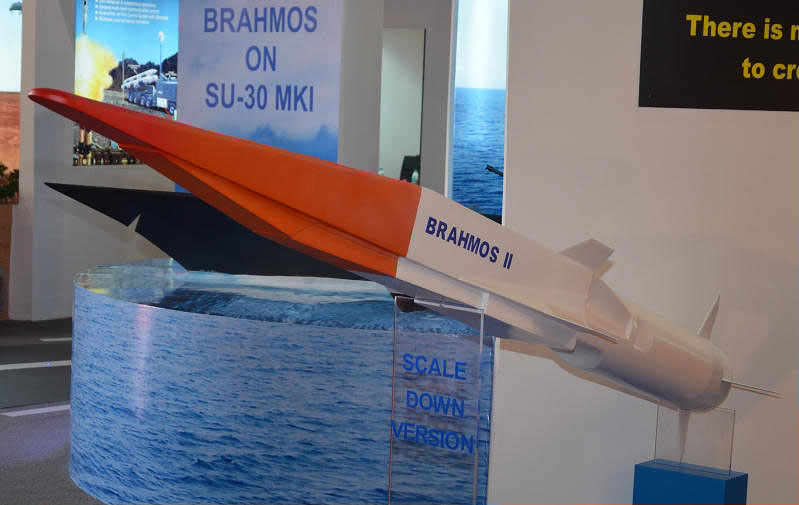
\includegraphics[width=\textwidth]{figures/brahmos-II}
		\caption{Maquette du missile hypersonique russo-indien BrahMos-II, en cours de développement. Crédit : Pakistan Defence (\url{http://defence.pk}).}
		\label{fig:brahmos}
	\end{figure}
	
	\paragraph{}
	En situation réelle, un espace aérien pourrait tout à fait contenir des véhicules et autres engins volants de tous les types sus-cités, des essaims de drones très manœvrables jusqu'aux missiles balistiques les plus rapides. Un système de contrôle interactif devrait donc être assez souple pour permettre la sélection de cibles de natures très différentes.
	On peut noter que les engins volants militaires ont vocation à chercher à éviter d'être détectés, soit en étant naturellement furtifs, soit en volant à très basse altitude et en tirant parti du relief naturel. Il en résulte qu'ils peuvent n'apparaître sur les écrans de contrôle que lorsqu'ils sont déjà très proches de lieux à protéger, et peuvent éventuellement disparaître de ces écrans, offrant une fenêtre temporelle restreinte pour l'interaction.
	
	\subsection{Observations}
	Qu'il s'agisse d'applications civiles ou militaires, cette tâche est critique, puisque de nombreuses vies sont en jeu. Selon l'application, il peut donc y avoir des contraintes fermes et spécifiques, soit sur le temps de sélection maximal acceptable (contrainte de temps-réel) soit sur le taux d'erreur, ou encore sur les niveaux de zoom, etc.

	Les systèmes de contrôle aérien dont nous avons connaissance sont tous en deux dimensions. Pour des engins volants, cela implique nécessairement une perte d'informations. Une technique de sélection suffisamment performante pourrait rendre envisageable l'utilisation d'un système en 3D. Cela permettrait par exemple de mieux déterminer si deux avions qui paraissent dangereusement proches dans le plan le sont réellement dans l'espace, ou de pouvoir choisir un objet parmi plusieurs évoluant aux mêmes coordonnées 2D, mais à des altitudes différentes, ou tout simplement d'avoir une meilleure représentation et perception générales de la situation.


	\begin{figure}[ht]
		\centering
		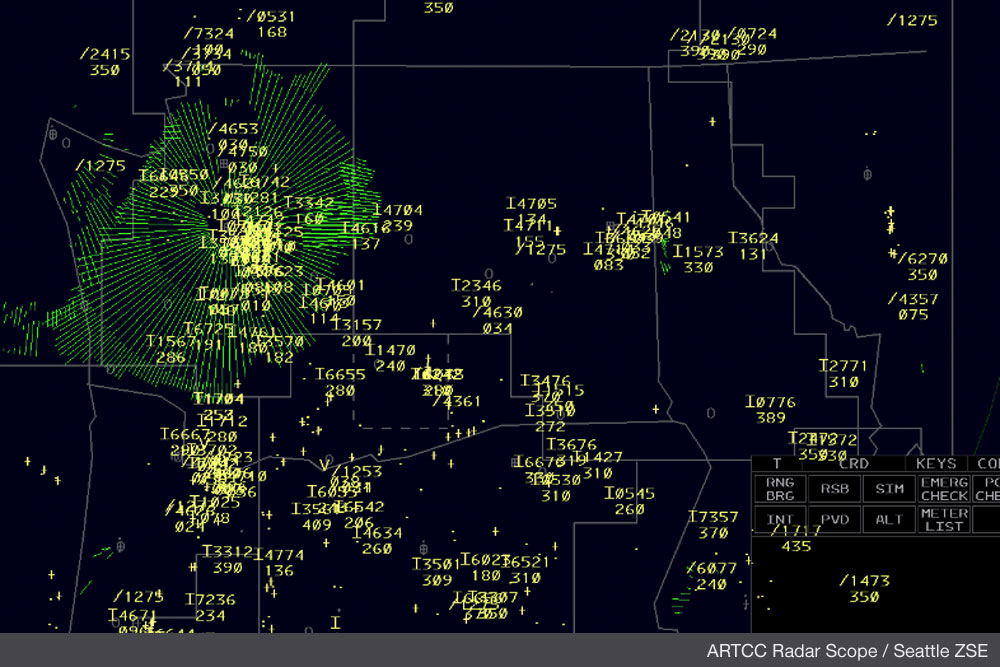
\includegraphics[width=\textwidth]{figures/Radar-Scope-ZSE}
		\caption{Écran de contrôle du trafic aérien. Crédit : www.boldmethod.com}
		\label{fig:airtraffic}
	\end{figure}
	
	\section{Vidéo-surveillance}
	La vidéo-surveillance s'applique aussi bien aux foules dans les lieux publics ou sensibles qu'à la voirie, où peuvent circuler des véhicules de types divers. Un agent de sécurité en charge de visionner un flux de vidéo-surveillance pourrait avoir à sélectionner une personne, par exemple pour obtenir des informations sur celle-ci grâce à la reconnaissance faciale, ou un véhicule, pour les mêmes raisons, par exemple grâce à sa plaque d'immatriculation. Quelle que soit la nature de la cible, sa sélection pourrait avoir pour but de zoomer dessus, de verrouiller une caméra robotisée afin qu'elle la suive, ou de la désigner à des forces de sécurité sur le terrain pour qu'elles interviennent physiquement.
	
	La vitesse d'un 
	Changements de direction très imprévisibles et totalement libres.
	
	Voitures : 0 à 130 km/h en cas normal, bien plus en course-poursuite
	Période de changements de direction de l'ordre de la dizaine de secondes, pouvant être de 90 degrés (voire plus) à basse vitesse, beaucoup plus progressifs à grande vitesse.
	
	\section{Analyse de processus complexes}
	
	\section{Retransmissions d'événements sportifs}
	Les retransmissions d'événements sportifs présentent un potentiel d'interactivité intéressant, nécessitant souvent la sélection de cibles mobiles. Il peut être intéressant, par exemple, de sélectionner un joueur de football pour afficher des statistiques. Pour les mêmes raisons, un ballon ou une balle peut être une cible, de même que certains éléments du terrain de jeu, qui sont physiquement fixes mais peuvent être mobiles à l'écran du fait des mouvements de caméra. La nature du mouvement de ces cibles varie nécessairement d'un sport ou d'un jeu à l'autre.
	
	Des sports d'équipe comme le football, le hockey sur glace ou le basket-ball sont caractérisés par des cibles potentielles relativement nombreuses, mobiles, et dont les mouvements ne sont pas toujours très prévisibles. Les courses athléthiques, hippiques, ou les sports mécaniques présentent des mouvement souvent plus prévisibles, mais aussi nettement plus rapides, avec en plus une certaine tendance des cibles à être très proches les unes des autres, ce qui augmente la probabilité d'erreur de sélection.
	
	Humains : 0 à 45 km/h
	Changements de direction très imprévisibles et totalement libres
	
	Paramètres beaucoup plus variables pour les projectiles, mais raccourci ?
	
	Cependant, dans la plupart 
	
	\section{Jeux vidéo}
	La sélection ou le pointage de cibles mobiles est une tâche que l'on retrouve dans de très nombreux jeux vidéo, appartenant à un nombre important de catégories. On peut notamment citer les jeux de tir (\emph{Fist-person Shooters}, ou FPS), les jeux de stratégie et tactique militaire (les catégories \emph{Real-time strategy} ou RTS, et \emph{Real-time tactics} ou RTT), les simulateurs de vol de combat (réalistes ou non) ainsi que les jeux de type arène de bataille en ligne multijoueur (\emph{Multiplayer online battle arena}, ou MOBA).
	
	
	
	\section{}
    
	Les tendances observées sur les cibles statiques demeurent, à savoir que la difficulté de la tâche augmente quand la distance entre la cible et le pointeur augmente, ou quand la taille de la cible diminue. Mais l'influence du mouvement de la cible empêche d'appliquer la loi de Fitts. Certes, la difficulté de la tâche augmente aussi avec la vitesse, [ref-mec-interact?] cependant, si la nature du mouvement a une importance cruciale, celle-ci demeure peu étudiée.
    
    
    
    
 The
difficulty of the selection increases while (1) target size decreases,
(2) target velocity increases and (3) target density increases. The
selection is even more difficult in 3D environments (filmed or synthetic
environments) because a target of interest can be occluded
by others targets. Selecting someone in crowds with a surveillance
video system is an example of a dense environment with small targets
and occlusion. In some cases, like in action sport footage, both
the objects of interest and the camera can move. Target movements
become unpredictable, and the selection is even more difficult.
In this context, as Hasan et al. [3] wrote, for completing the
selection ”the user must continually track the target and simultaneously
plan to move the cursor over it”. This underscores the key
point of the technique we propose here. Since the user follows the
target for selecting it, the Hook technique tracks the cursor behavior
for assisting the selection. Indeed, observing the history of cursor
displacements, and the history of distances between each target and
the cursor, the system can estimate which target is tracked, and then
propose a selection to the user who just has to validate it. In other
words, the user follows the target of interest, and the system will
know which target it is.
This paper presents the implementation of this technique, and
two experiments which investigate its performance. Hook has been
compared to the basic pointing (non assisted pointing), and to Bubble
cursor [2, 8], for the case of 3D object selection. The first evaluation
involves a desktop configuration, in which pointing is done
on a standard screen with a mouse. The second evaluation involves
an immersive configuration in which pointing is done with a 3dof
(degrees-of-freedom) device. Both evaluations highlight the bene-
fits of this new interaction technique for selecting moving targets in
a 3D environment. More than simply improving the pointing time,
Hook drastically decreases the error rate and allows pointing targets
in high density environments, with high velocity targets that are not
possible to capture with other techniques.


	
		

\clearpage
